\documentclass[a4paper,12pt]{report}

\usepackage{graphicx}
\usepackage[utf8]{inputenc}
\usepackage{hyperref}
\usepackage[left=2cm,right=2cm,top=2cm,bottom=2cm]{geometry}

\usepackage{lipsum}% http://ctan.org/pkg/lipsum
\usepackage{titletoc}% http://ctan.org/pkg/titletoc
\titlecontents*{chapter}% <section-type>
  [0pt]% <left>
  {}% <above-code>
  {\bfseries\chaptername\ \thecontentslabel\quad}% <numbered-entry-format>
  {}% <numberless-entry-format>
  {\bfseries\hfill\contentspage}% <filler-page-format>



\begin{document}

\graphicspath{{images/}}


\title{2nd Report \\ \textbf{Face Detection Techniques And Algorithms}}
	\author{----------------------------- \\   \\  \\   \\   \\   \\  \\   \\   \\   \\   \\ \textbf{Supervised by:}\\ Prof. Oussama El Issati\\ \textbf{Prepared by:} \\ Ait Said Noureddine \\ Ennouali Mohamed Amine}
	\maketitle



\maketitle

\tableofcontents


%\begin{abstract}


%\end{abstract}

\chapter{Face detection techniques and algorithms}
  \section{Introduction}
    Object detection is a computer technology related to computer vision and image processing that deals with detecting instances of semantic objects of a certain class (such as humans, buildings, or cars) in digital images and videos. Well-researched domains of object detection include face detection and pedestrian detection. Object detection has applications in many areas of computer vision, including image retrieval and video surveillance. \par
    Object detection algorithms are used in face detection and face recognition. It is also used in tracking objects, for example tracking a ball during a football match, tracking movement of a cricket bat, tracking a person in a video.\par
    The concept is that every object class has its own special features that helps in classifying the class – for example all circles are round. Object class detection uses these special features. For example, when looking for circles, objects that are at a particular distance from a point (i.e. the center) are sought. Similarly, when looking for squares, objects that are perpendicular at corners and have equal side lengths are needed. A similar approach is used for face identification where eyes, nose, and lips can be found and features like skin color and distance between eyes can be found\cite{wiki_link}.\par

\section{Face detection algorithms}
    Cascading is an ensemble learning based on the concatenation of several Classifiers, using all information collected from the output from a given classifier as additional information for the next classifier in the cascade. Cascading is a multistage system.\par
    Cascading classifiers are trained with several hundred ``\emph{positive}'' sample views of a particular object and arbitrary ``\emph{negative}'' images of the same size. \par
    After the classifier is trained it can be applied to a region of an image and detect the object in question. To search for the object in the entire frame, the search window can be moved across the image and check every location for the classifier. This process is most commonly used in image processing for object detection and tracking, primarily facial detection and recognition.\par

\subsection{Cascade classification based algorithm: Viola and Jones}
   The first cascading classifier is the face detector of \emph{Viola and Jones (2001)}. The requirement was that the classifier be fast in order to be implemented on low CPU systems, such as cameras and phones\cite{wiki_link}.\par
  \begin{figure}[h]
    \centering
    \caption{\label{cascade_concept} Concept of cascade classification\cite{haar_lbp_hog_comp_pdf}}
    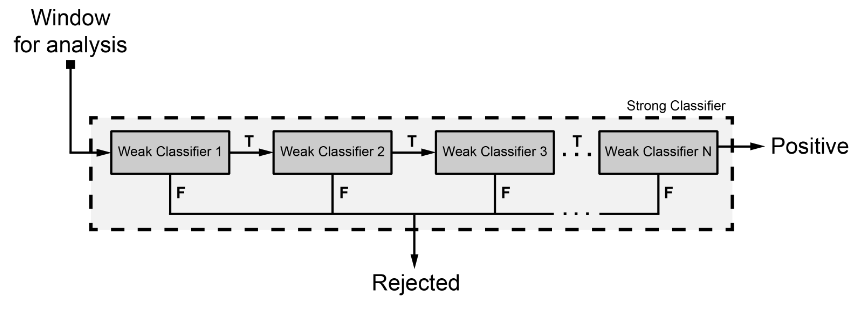
\includegraphics[scale=0.55]{cascade_concept.png}
  \end{figure}

\subsubsection{Characteristics of the algorithm}

  \begin{itemize}
      \item \textbf{Robust:} the algorithm has a very high detection rate (true-positive rate) and very low false-positive rate\footnotemark.
      \item \textbf{Real Time:}  At least 2 frames per second are processed thus making it a quick and an efficient algorithm. The algorithm comprises of four stages: 


      \begin{enumerate}
	\item Haar Features Selection 
	\item Creating Integral Image
	\item Adaboost Training Algorithm 
	\item Cascade Classifiers 
      \end{enumerate}

  \end{itemize}

\subsubsection{HAAR Features}
      Haar-like features are digital image features used in object detection\cite{viola_jones}. Haar features are similar to convolution 
      kernels which are used to detect the presence of a feature in the given image. 

%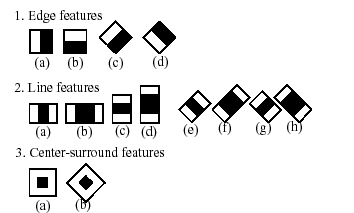
\includegraphics{haar_features.jpg}

      \begin{figure}[h]
	\centering
	\caption{\label{haar_feature} Haar features applied to detect faces\cite{opencv_website}.}
	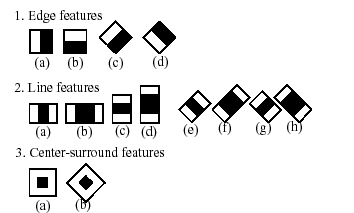
\includegraphics[scale=0.62]{haar_features.png}
	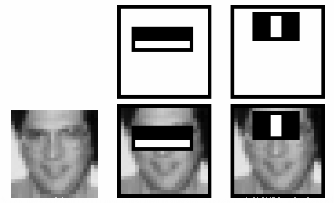
\includegraphics[scale=0.62]{haar_applied.png}
      \end{figure}

      A Haar-like feature considers adjacent rectangular regions at a specific location in a detection window, sums up the pixel intensities in each region and calculates the difference between these sums. \cite{opencv_website}\par
      There is a huge number of possible sizes and locations of each kernel. For example using a 24x24 window results over 160000 features. For each feature calculation, we need to find sum of pixels under white and black rectangles. To solve this, they introduced the integral images to simplify calculation of sum of pixels\cite{sonia_pdf}.

%Dans la figure~\ref{haar_feature} page~\pageref{haar_feature}

\subsubsection{Integral image}
      he  algorithm  introduces  the 
      concept of integral image to find the sum of all the pixels under a rectangle with just 4 corner values instead of 
      summing  up all the values.

\subsubsection{Adaboost}
      Since not all the features are relevant, we have to select only the best features using Adaboost. Which is  a  machine  learning  algorithm  which  helps  in  finding  only  the  best  features  among  all  the 
      160000+ features. After  these  features  are  found,  a  weighted  combination  of  all  these  features  is  used  in 
      evaluating  and  deciding  if  any  given  window  (24x24)  has  a  face  or  not.  Each  of  the  selected  feature  is 
      considered to be included if they can at least perform better than random guessing. The little classifiers are called ``weak classifiers'', Adaboost  constructs  a  strong  classifier  as  a  linear 
      combination of these weak classifiers.

\subsubsection{HAAR classifier generating}
      The process of generating a classifier includes two stages: the training and the detection stage. The detection stage using either HAAR or LBP based models. The library \textbf{OpenCV} comes with preprogramed applications that we can use to generate a classifier in $.xml$ file, this file contains all the features that will be used to look for faces in future applications, OpenCV comes also with pre-generated $.xml$ files ready to use.

      \begin{figure}[h]
	\centering
	\caption{\label{haar_stage_vis} The process of classifier generation using OpenCV.}
	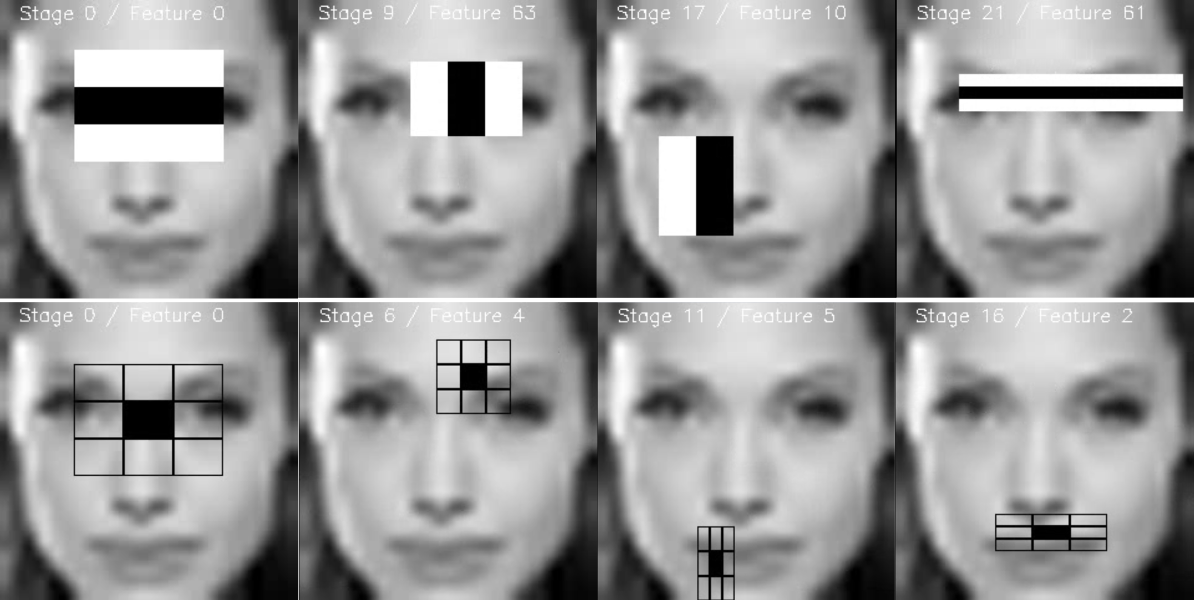
\includegraphics[scale=0.5]{haar_stage_vis.png}
      \end{figure}

\subsubsection{Advantages}

      \begin{itemize}
      \item Fast features are computed very quickly. 
      \item The features are scaled instead of scaling the image. 
      \item This is a generic detection scheme which can be used to detect other objects like hands, buildings, etc. 
      \end{itemize}

\subsubsection{Disadvantages}

      \begin{itemize}
	\item The detector is effective only in the case of frontal images of the face. 
	\item If the face is turned 45 degrees, it fails to detect the face. 
	\item It is sensitive to lighting conditions.
	\item Due  to  overlapping  sub-windows,  we  might  face  the  problem  of  multiple  objects  being  detected  as face. 
      \end{itemize}

\subsubsection{Results}

      \begin{figure}[h]
	\centering
	\caption{\label{haar_result} Default OpenCV HAAR cascade classifier test.}
	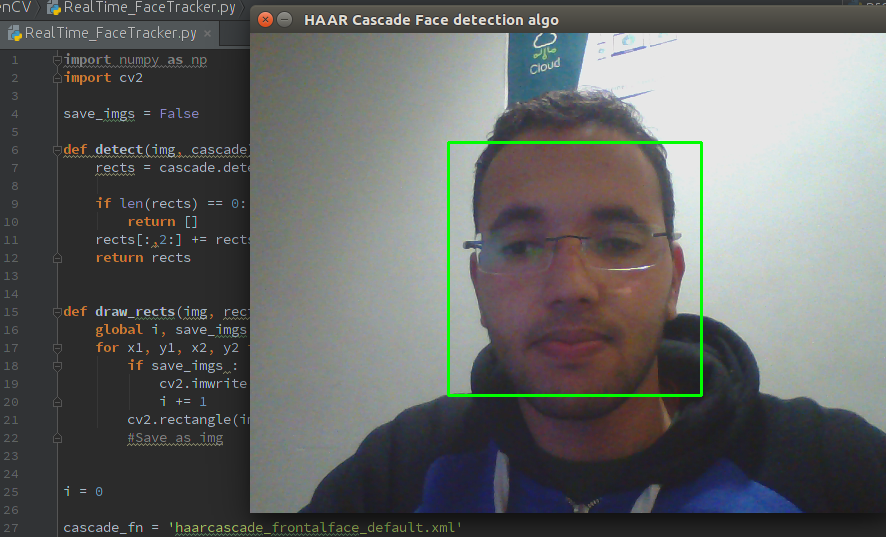
\includegraphics[scale=0.5]{haar_test.png}
      \end{figure}


\subsection{CAMshift Algorithm}
    CAMshift is a tracking algorithm, which is based on MeanShift algorithm, what CAMshift does meanShift in every single frame of a video, and record the results we got by MeanShift. 
    CamShift algorithm includes these three parts\cite{camshift} :
    
      \begin{enumerate}
	\item Back projection 
	\item Applying MeanShift
	\item Tracking
	    
      \end{enumerate}
  
  \subsubsection{Back Projection}
  
  Back projection is a method using the histogram of an image to show up the probabilities of colors that may appear in each pixel.
First we transform the picture space to HSV space which is a cylindric color base (or any space which include an H channel that represent the hue of each pixel, of course, value of hue is between 0 to 180). Secondly, we split the H channel out, as a single grayscale image, and get its histogram, and normalize it. Thirdly, we use “calcBackProject()” function to calculate the back projection of the image.

  \textbf{Example:} 
  
This is an example to explain how we get the back projection.   We transform the picture into HSV space and the second image shows the hue channel. The third image shows its histogram.
We calculate the weight of each color in the whole picture using histogram, and change the value of each pixel to the weight of its color in whole picture, the result of this step is shown in the last image.
  \begin{figure}[h]
    \centering
    %\lefting
    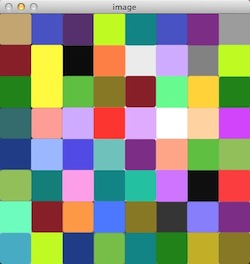
\includegraphics[scale=0.55]{backpro1.jpeg}
     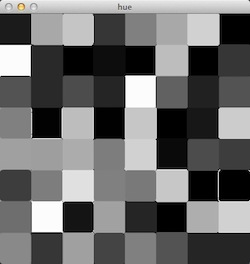
\includegraphics[scale=0.55]{backpro2.jpeg}
     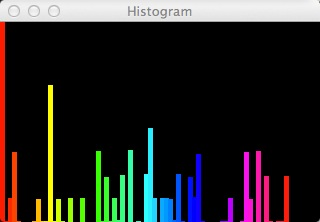
\includegraphics[scale=0.62]{backpro3.jpg}
     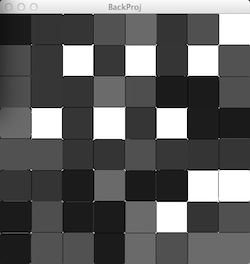
\includegraphics[scale=0.55]{backpro4.jpeg}

  \end{figure}
  
  
  \subsubsection{Applying MeanShift}
  
  MeanShift is an algorithm which finding modes in a set of data samples representing an underlying probability density function, so the whole algorithm is:

      \begin{enumerate}
	\item Initialize the sphere, including the center and radius.
	\item Calculate the current mass center.
	\item Move the sphere’s center to mass center
	\item Rrepeat step b and c, until converge, that is, current mass center after calculate, is the same point with center of sphere.
	    
      \end{enumerate}
  
  \begin{figure}[h]
    \centering
    %\lefting
    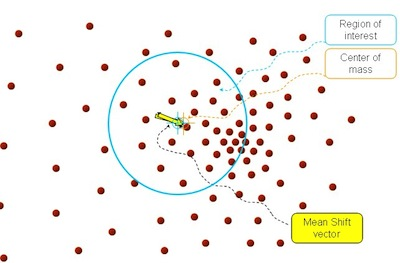
\includegraphics[scale=0.7]{meanshift2.jpg}
    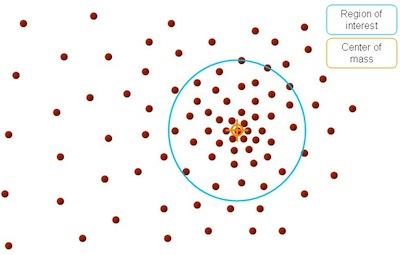
\includegraphics[scale=0.7]{meanshift3.jpg}
    \caption{The meanshift method.}

  \end{figure}
  
    \subsubsection{Track}

    The last step is tracking, if we have a video, or frames captured by our web camera, what we need to do is just use meanShift algorithm to every single frame, and the initial window of each frame is just the output window of the prior frame.
  

\begin{thebibliography}{9}
  \bibitem{wiki_link} 
    \textit{Wikipedia}.\\
    \url{https://en.wikipedia.org/wiki/Object_detection} \\
    \url{https://en.wikipedia.org/wiki/Computer_vision}
    
  \bibitem{viola_jones}
    P. Viola,  M.J. Jones
    \textit{``Robust  Real-Time  Face  Detection,  International Journal  of  Computer Vision''}, Vol.  57, No. 2, May 2004.
    
  \bibitem{sonia_pdf}
    \textit{``Face Detection and Tracking: A Comparative Study Of Two Algorithms''}
    Sonia Mittal, Chirag Shivnani\\
    \url{http://csjournals.com/IJCSC/PDF7-1/11.\%20Sonia.pdf}
    
    \bibitem{opencv_website}
    \textit{OpenCV Documentation Website} \\
    \url{https://opencv-python-tutroals.readthedocs.io/en/latest/py_tutorials/py_tutorials.html}\\
    \url{http://docs.opencv.org/3.1.0/db/df8/tutorial_py_meanshift.html}
    
    
   \bibitem{haar_lbp_hog_comp_pdf}
    \textit{``A comparison of Haar-like, LBP and HOG approaches to concrete and asphalt
runway detection in high resolution imagery''} \\
    \url{http://epacis.net/jcis/PDF_JCIS/JCIS11-art.0101.pdf}
    
    \bibitem{camshift}
    \textit{``Continuously Adaptive Shift''} \\
    \url{http://eric-yuan.me/continuously-adaptive-shift/}
    


\end{thebibliography}



\end{document}          
